\documentclass{article}
\PassOptionsToPackage{numbers,compress}{natbib}
\usepackage[dblblindworkshop]{neurips_2026}
\workshoptitle{AXIOM}
\usepackage[utf8]{inputenc}
\usepackage[T1]{fontenc}
\usepackage{hyperref}
\usepackage{url}
\usepackage{booktabs}
\usepackage{amsfonts,amsmath,amssymb}
\usepackage{nicefrac}
\usepackage{microtype}
\usepackage{graphicx}
\usepackage{xcolor}
\usepackage{caption}
\captionsetup{font=small,labelfont=bf}
\graphicspath{{../figs/}}

\title{Superposition Is Free to Quantize: Precision Cost Is Set by Outliers and Feature Margins, Not Feature Density}

\author{Anonymous Author(s)}

\begin{document}
\nolinenumbers
\maketitle

\begin{abstract}
Networks store more features than dimensions by superposing them as non-orthogonal directions, and a direction is only
as resolvable as the grid it is stored on---so a layer doing more superposition should need more bits. We preregistered
that hypothesis as a closed-form law (half a bit per doubling of features-per-dimension $F$) and tested it in 2{,}100
toy models of superposition, against five non-quantization damage families, and inside GPT-2 small. It is wrong:
the critical bit-width is flat in $F$ over a $14\times$ range (slope $-0.11$, CI $[-0.12,-0.09]$). What sets it is a
tolerance to relative weight perturbation that is independent of $F$ and shared, within a factor of two, by rounding,
dithering, stochastic rounding and Gaussian noise, together with the outlier ratio $\kappa=\max|W|/\mathrm{rms}(W)$, which
enters as $\log_2\kappa$---causally in the toy model (clipping $\kappa$ moves the bit-width, $R^2=0.92$), across GPT-2's 48 weight matrices
($R^2=0.53$, slope $0.6$--$0.7$, of which a quantizer-free noise arm predicts $0.54$ [$0.35$, $0.71$]) and for their input
activations, where the activation outlier ratio sets activation bits with slope $1.12$ [$0.91$, $1.39$], $R^2=0.73$. In an exploratory follow-up the half-bit-per-doubling exponent reappears one level down: a feature's critical
bit-width follows its own fp32 margin, in the toy model ($R^2=0.68$, 4{,}290 features), for GPT-2's next-token predictions
(logit margin, not rarity; $R^2 = 0.23$ per token, $0.90$ binned) and for 22{,}499 sparse-autoencoder features ($R^2=0.45$
per feature, $0.94$ binned). Quantization deletes a model's weakest features first, in an order that a one-number
statistic predicts.
\end{abstract}

\section{Introduction}
Superposition---packing more features than dimensions as nearly orthogonal directions~\cite{elhage2022toy}---is the
prevailing account of how networks represent sparse features, and every quantitative treatment of it assumes
infinite-precision weights. Quantization is the practice of storing those weights on a coarse grid. The two have never
been connected, yet a connection is natural: a direction is only as resolvable as the grid it is stored on, so a layer
that superposes more features per dimension ($F$) should need more bits---an intuition entertained, without controls, in
the one prior experiment on the question~\cite{bitnets}, and one we found compelling enough to preregister. If true, it
would convert a mechanistic quantity into an engineering one (a critical bit-width) and give a representational account
of the weight-outlier counterpart of the folklore that outliers make layers hard to quantize~\cite{dettmers2022,xiao2023,lin2024awq}.

We made the intuition precise and \emph{preregistered} it (Sec.~\ref{sec:setup}): $b_{\mathrm{crit}} = 1 +
\log_2(1+\kappa\sqrt{F/3})$, half a bit per doubling of $F$, with decision bands, controls and a real-model bridge committed
before any experiment ran. Our contributions:
\begin{itemize}\setlength\itemsep{1pt}
\item \textbf{The intuition is wrong.} Across 40 toy configurations spanning $F = 4$--$56$, under both
quantization-aware and post-training quantization, the critical bit-width is flat in $F$ (slope $-0.11$
[$-0.12$, $-0.09$]); in GPT-2 a superposition proxy predicts nothing ($R^2=0.04$). A corrected derivation explains why:
at high $F$ the interference quantization adds must be compared with the interference already present, and $F$ cancels.
\item \textbf{What sets the bit-width.} A tolerance to relative weight perturbation that is independent of $F$ and
shared within $2\times$ by five damage families, and the outlier ratio $\kappa$, which enters as $\log_2\kappa$: causally
in the toy model (clipping $\kappa$ at fixed configuration moves $b_{\mathrm{crit}}$ with $R^2=0.92$) and in GPT-2's 48
matrices ($R^2=0.53$). The tolerance itself grows as $\kappa^{0.46}$ (measured with Gaussian noise, no quantizer involved), which predicts an
RTN slope of $0.54$ [$0.35$, $0.71$]; the RTN slope measured independently is $0.63$ [$0.49$, $0.75$]---consistent within
error, with the prediction $0.1$ low. The same law holds for
activations (post hoc): each matrix's activation bit-width follows its activation outlier ratio with slope $1.12$
[$0.91$, $1.39$], $R^2=0.73$. Per-channel scaling removes the weight-$\kappa$ tax (all 48 matrices at $2.7\pm0.3$ bits), so
a $\kappa$-based allocator does not beat uniform per-channel quantization.
\item \textbf{A per-feature law (exploratory, not preregistered).} The half-bit-per-doubling exponent is real at the
feature level: a feature's critical bit-width follows its fp32 margin, in toy models ($R^2=0.68$), for GPT-2 next-token
predictions (margin beats rarity; $R^2=0.23$ per token, $0.90$ binned) and for GPT-2's internal sparse-autoencoder
features ($R^2=0.45$ per feature, $0.94$ binned, $n=22{,}499$). This is a candidate mechanism for the tail-loss
phenomenon of compressed models~\cite{hooker2019,hooker2020}, found after the preregistered analyses and reported as such.
\end{itemize}

\begin{figure}[t]
\centering
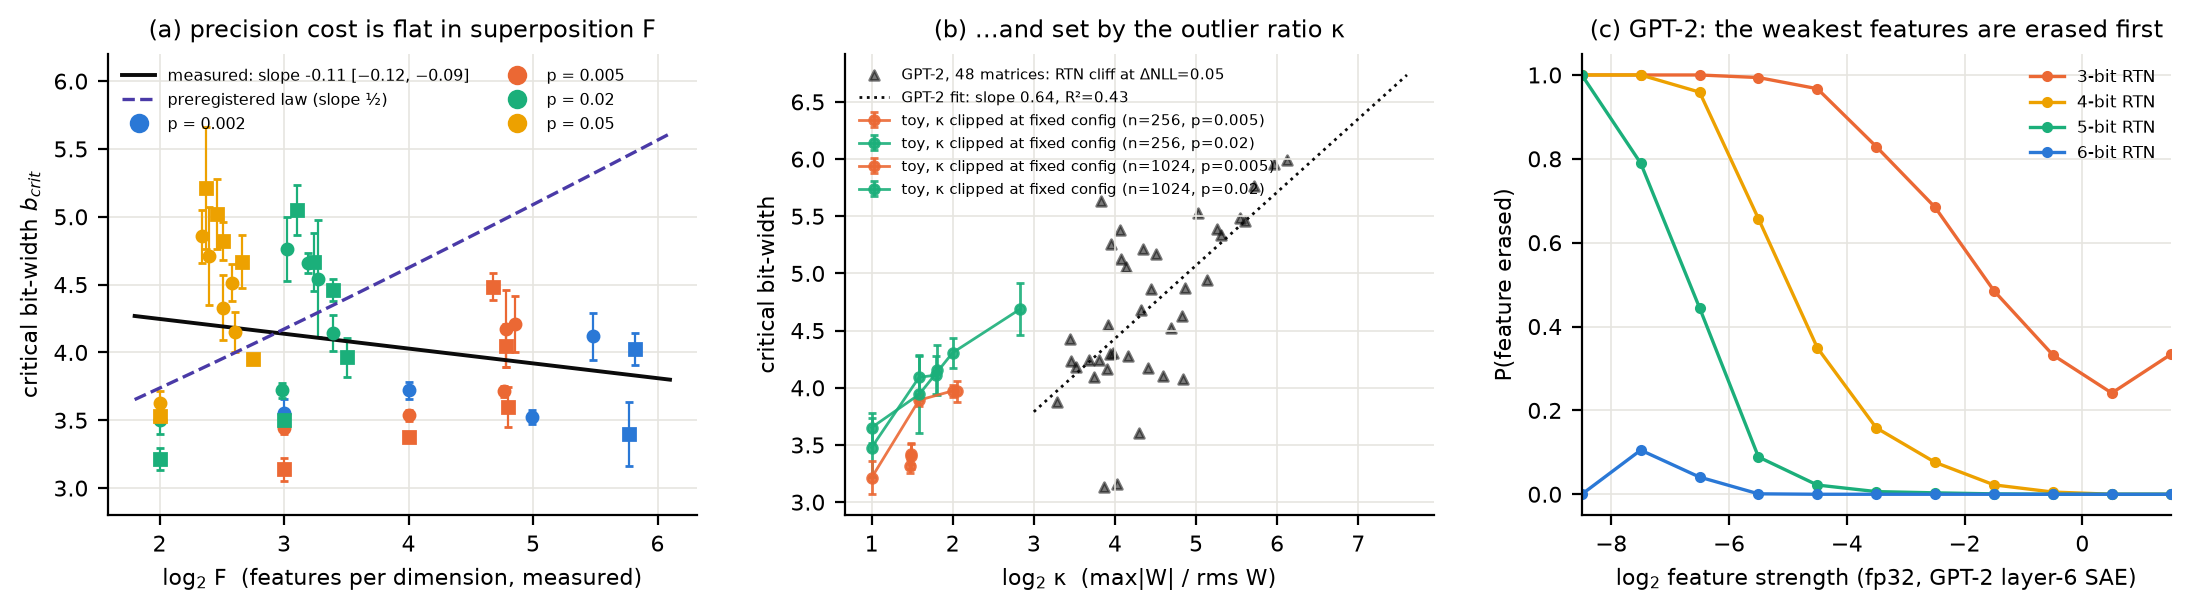
\includegraphics[width=\linewidth]{fig_hero.png}
\caption{\textbf{(a)} Critical bit-width (RTN, QAT, 95\,\% retention; mean $\pm$ SD over 4 seeds) against measured
features-per-dimension for the main sweep, with the preregistered law. \textbf{(b)} $b_{\mathrm{crit}}$ against
$\log_2\kappa$: toy models with $\kappa$ moved by weight clipping at fixed configuration, and GPT-2's 48 matrices (each
quantized alone, per-tensor RTN, threshold $\Delta\mathrm{NLL}=0.05$). \textbf{(c)} Fraction of GPT-2 layer-6
sparse-autoencoder features whose activation pattern is lost when blocks 0--5 are quantized jointly, by feature strength.}
\label{fig:hero}
\end{figure}

\section{Setup, the preregistered law, and why it fails}
\label{sec:setup}
\textbf{Model.} Tied-weight toy models of superposition~\cite{elhage2022toy}: $x\in\mathbb{R}^n$ with feature $i$ active
with probability $p$ and value $\sim U[0,1]$; $h=Wx$, $W\in\mathbb{R}^{m\times n}$; $\hat x=\mathrm{ReLU}(W^\top h+b)$;
squared-error loss with importance $I_i$. Writing $W_i$ for column $i$, $\hat x_i = \mathrm{ReLU}(\lVert W_i\rVert^2x_i +
\sum_{j\neq i}(W_i^\top W_j)x_j + b_i)$: the sum is the interference superposition costs. Per feature we measure
$\rho_i = 1-\nu_i/\nu_i^0$ ($\nu_i$ the reconstruction error, $\nu_i^0$ that of the best constant); a column is \emph{live}
if $\lVert W_i\rVert\ge0.5$ (norms are bimodal); $F = k/m$ with $k$ the live count of the fp32 model. Retention at
bit-width $b$ is $R(b) = \sum_{i\in\mathrm{live}}\rho_i(b)/\sum_{i\in\mathrm{live}}\rho_i(\infty)$ on identical samples,
and $b_{\mathrm{crit}}$ is the interpolated width at which $R = 0.95$ ($b=2$ never fitted; 90/99\,\% as sensitivity).

\textbf{Quantizer.} Per-tensor symmetric round-to-nearest (RTN), $q_{\max}=2^{b-1}-1$, $\Delta=\max|W|/q_{\max}$, applied
once to $W$ and used in both directions, trained through a straight-through estimator (QAT) or applied post-training
(PTQ); also dithered, stochastic-rounding and per-channel variants. The residual $\varepsilon = Q(W)-W$ is always measured.

\textbf{The preregistered law.} With unit live columns, tied weights double the cross-talk, only live columns interfere
(dead columns round to exactly 0), and $\max|W| = \kappa\,\mathrm{rms}(W)$ grows with occupancy. Summing the
quantization-induced cross-talk over $k$ live interferers active with probability $p$ gives an added interference
variance $p\kappa^2k^2/(18\,mn\,q_{\max}^2)$; equating it to the retention threshold $\nu^0/2$ and using $n\approx k$
yields $q_{\max,\mathrm{crit}} = \kappa\sqrt{F/3}$, i.e.\ $b_{\mathrm{crit}} = 1+\log_2(1+\kappa\sqrt{F/3}) \approx
\mathrm{const}+\tfrac12\log_2F$. The slope $\nicefrac12$ was the claim (bands: $[0.4,0.6]$ confirmed; $<0.15$ dead).

\textbf{Why it fails} (recorded after a sizing pilot, before the main sweep; App.~\ref{app:deviations}). The derivation
compares the \emph{added} interference with the explainable variance. But at $F\gg1$ the fp32 model already carries
interference many times that---the Welch bound gives $\sum_{j\neq i}(W_i^\top W_j)^2 \gtrsim F-1$---and survives it
through the ReLU with a strongly negative bias. The loss responds to added cross-talk \emph{relative to existing}
cross-talk: per pair $2\sigma_\varepsilon^2$ against $1/m$, a ratio $2m\sigma_\varepsilon^2 =
\lVert Q(W)-W\rVert_F^2/\lVert W\rVert_F^2 = \sigma_{\mathrm{rel}}^2$, the squared relative perturbation of each feature
direction. $F$ cancels. Since the residual lives on the live columns, $\sigma_{\mathrm{rel}} =
\kappa_{\mathrm{live}}/(\sqrt{12}q_{\max})$ with $\kappa_{\mathrm{live}} = \max|W|/\mathrm{rms}(W_{\mathrm{live}})$, so the
corrected prediction is $\sigma_{\mathrm{rel,crit}}$ independent of $F$ and
\begin{equation}
b_{\mathrm{crit}} \approx 1+\log_2\!\big(1+\kappa_{\mathrm{live}}/(\sqrt{12}\,\sigma_{\mathrm{rel,crit}})\big) = \mathrm{const} + \log_2\kappa_{\mathrm{live}} .
\label{eq:corrected}
\end{equation}
The algebra is the uniform-quantizer noise formula inverted; the empirical content is the claim that
$\sigma_{\mathrm{rel,crit}}$ is a property of the representation that does not depend on how densely features are packed.
We do not claim it is a universal constant: below we measure how it varies across damage types and with $\kappa$, and use
the measured dependence in Eq.~\eqref{eq:corrected}.

\section{Results}
All toy models: Adam $10^{-3}$, 200-step warm-up, cosine decay, 6000 steps, fp32 on Apple MPS; $\ge$40k evaluation
samples with the quantizer active; every arm of a (configuration, seed) shares data and evaluation samples (paired).
Every mean carries a seed SD or a seed-bootstrap CI (App.~\ref{app:methods}).

\textbf{Flat in $F$ (E1, E3).} The main sweep ($m\in\{10,16\}$, $n/m\in\{4,\dots,128\}$, $p\in\{0.002,\dots,0.05\}$,
$b\in\{2,\dots,8,\infty\}$, 4 seeds, 1536 models) gives Fig.~\ref{fig:hero}a: over 40 cells with $F = 4.0$--$56.5$
and $\kappa = 2.5$--$13.5$, $b_{\mathrm{crit}}$ is $3.1$--$5.2$ bits and its slope in $\log_2F$ is $-0.11$
[$-0.12$, $-0.09$] (90\,\%: $-0.15$; 99\,\%: $+0.04$; hard count where defined: $-0.27$). Post-training RTN on the same
models: $3.87\pm0.15$ bits in every cell, slope $+0.03$ [$0.02$, $0.04$]. In GPT-2 small (48 matrices, one damaged
at a time, App.~\ref{app:lm}) the noise threshold has no relation to a superposition proxy $\hat F = d_{\mathrm{in}}/\mathrm{PR}$
(slope $+0.14$ [$-0.13$, $0.35$], $R^2=0.04$).

\textbf{An $F$-independent tolerance (E3).} Applying seven damage families post-hoc to the same fp32 models on a common axis
$\sigma_{\mathrm{rel}} = \lVert D(W)-W\rVert_F/\lVert W\rVert_F$: RTN, per-channel RTN, dithered and stochastic rounding
and Gaussian noise all cost 5\,\% of the represented features' explained variance at $\sigma_{\mathrm{rel}}\approx
0.10$--$0.23$, flat in $F$ (slopes $0.00$--$0.05$ against the predicted $-\nicefrac12$; 44 cells), and their retention
curves collapse against $\sigma_{\mathrm{rel}}$. Structured damage differs (dropout tolerated to $0.3$--$0.5$; rank truncation catastrophic).

\textbf{Outliers set the bit-width (E6, GPT-2).} Across the sweep $b_{\mathrm{crit}} = 2.0+0.72\log_2\kappa$ ($R^2 = 0.82$;
$b_{\mathrm{crit}}-\log_2\kappa = 1.99\pm0.31$). Because $\kappa$ and the live fraction are collinear there, we moved
$\kappa$ directly: clipping weights at $c\cdot\mathrm{rms}(W)$ at fixed $(m,n,p)$ takes $\kappa$ from $7.1$ to $2.0$ and
$b_{\mathrm{crit}}$ from $4.69$ to $3.65$; pooled within-cell slope $0.65$, $R^2=0.92$ (Fig.~\ref{fig:hero}b).
In GPT-2 the independently measured per-tensor RTN cliff of each matrix follows $\log_2\kappa$ with slope $0.63$
[$0.49$, $0.76$], $R^2 = 0.53$, against $R^2=0.14$ for $\hat F$ (joint: $2.40+0.72\log_2\kappa-0.12\log_2\hat F$), and
converting each matrix's Gaussian-noise threshold to bits with Eq.~\eqref{eq:corrected} reproduces its RTN cliff with a
mean error of $-0.23$ bits. The slope is $0.6$--$0.7$ rather than $1$ in all three settings. A non-circular test of why: $\sigma_{\mathrm{crit}}$ is
measured from the Gaussian-noise arm and involves no quantizer, and across the GPT-2 matrices it grows with the outlier
ratio, $\sigma_{\mathrm{crit}}\propto\kappa^{e}$ with $e = 0.46$ [$0.29$, $0.65$] ($R^2=0.35$; outlier-heavy tensors carry
their function in a few large entries that a unit of relative noise moves less). Substituted into
Eq.~\eqref{eq:corrected} this predicts an RTN slope of $1-e = 0.54$ [$0.35$, $0.71$]; the slope measured independently
from the RTN arm is $0.63$ [$0.49$, $0.75$], a paired difference of $+0.09$ [$-0.05$, $+0.26$] (replicated at $\Delta\mathrm{NLL}=0.02$, App.~\ref{app:lm}):
consistent within error, central value $0.1$ low, so the account explains part of the shortfall, not all. $\sigma^*$ is
not a constant but a smooth function of $\kappa$ that is flat in $F$. With per-channel scaling the pathology
disappears and every GPT-2 matrix crosses the threshold at $2.70\pm0.33$ bits, uncorrelated with $\kappa$ or $\hat F$;
consequently mixed precision has little left to gain: uniform per-channel RTN is within $0.01$--$0.02$ nats of a
sensitivity oracle at 4 and 5 bits, and a $\kappa$-based allocation is \emph{worse} than uniform there (App.~\ref{app:lm},
Table~\ref{tab:mixed}). Only a per-matrix noise probe matches the oracle, and only between integer budgets. Dithered quantization is \emph{worse} than the shared lattice ($+0.27\pm0.13$ bits under QAT) because it moves
the exact zeros of dead columns off the lattice; stochastic rounding is worse still ($+0.63\pm0.11$).

\textbf{The per-feature law (E5, GPT-2; exploratory).} Under power-law importance $I_i=(i+1)^{-\alpha}$ the toy model drops features
from the tail, and quantization respects the order (prefix fraction $0.95$--$0.99$ at every $b\ge3$ vs $0.96$--$0.98$ at
fp32). The ten most important features need 3 bits in every configuration, the marginal ones 4--8; across all 4{,}290
live features the critical bit-width follows the feature's fp32 margin above the retention threshold, $b_i = c -
0.52\log_2(\rho_i^{\mathrm{fp32}}-\tfrac12)$, $R^2 = 0.68$. The same law holds inside GPT-2 twice. For next-token
predictions (all 48 matrices quantized jointly, per-channel RTN, 49k held-out tokens): at 4 bits, tokens with an fp32
logit margin below $\nicefrac18$ flip 58\,\% of the time, margin 1--2 logits 9\,\%, margin above 8 logits 0.5\,\%; the
critical bit-width falls with $\log_2$ margin at slope $-0.34$ per token ($R^2=0.23$; individual tokens are noisy) and
$-0.39$ for the binned means ($R^2=0.90$), and margin dominates rarity
($b_t = 5.30-0.36\log_2\mathrm{margin}-0.09\log_2\mathrm{freq}$). For internal features, using a public sparse autoencoder on
the residual stream entering block 6 (24{,}576 features, 84\,\% variance explained on our text) and quantizing blocks 0--5
jointly: 26/84/99\,\% of the 22{,}499 live features survive 3/4/5 bits, and which ones are erased is set by their
strength (Fig.~\ref{fig:hero}c)---features contributing $2^{-7}$ of the residual rms need $5.5$--$6$ bits, features at
$2^{0}$ survive at 3; per-feature slope $-0.37$ [$-0.38$, $-0.37$] ($R^2 = 0.45$ per feature, $0.94$ binned), with
frequency adding nothing ($+0.02$). Gaussian noise gives the same curves in every case.


\begin{table}[h]\centering\footnotesize
\caption{Key results (CIs: seed bootstrap for toy models, matrix bootstrap for GPT-2; ``prereg.'' = preregistered value;
``P2 form'' = P2's functional form applied post hoc to a new arm, not preregistered coverage; rows marked exploratory were not preregistered).}
\label{tab:key}
\setlength{\tabcolsep}{4pt}
\resizebox{\linewidth}{!}{\begin{tabular}{llll}\toprule
question & quantity & result & prereg.\\\midrule
does $F$ set bits? & $b_{\mathrm{crit}}$ slope in $\log_2F$, QAT / PTQ & $-0.11$ [$-0.12,-0.09$] / $+0.03$ [$0.02,0.04$] & $+0.5$\\
does $\kappa$ set bits? & within-cell slope in $\log_2\kappa$, $\kappa$ clipped (E6) & $0.65$, $R^2=0.92$ & $1$\\
 & GPT-2 RTN cliff vs $\log_2\kappa$ / vs $\log_2\hat F$ & $0.63$, $R^2=0.53$ / $0.28$, $R^2=0.14$ & --\\
 & GPT-2 activation bits vs $\log_2\kappa_{\mathrm{act}}$ / vs $\log_2\kappa_w$ (post hoc) & $1.12$ [$0.91,1.39$], $R^2=0.73$ / $0.35$, $R^2=0.12$ & P2 form\\
$F$-independent tolerance? & $\sigma_{\mathrm{rel,crit}}$ slope in $\log_2F$, five noise families & $0.00$ to $0.05$ & $-0.5$\\
which features die? (exploratory) & toy: $b_i$ vs $\log_2$ margin ($n=4290$) & $-0.52$, $R^2=0.68$ & --\\
 & GPT-2 tokens: $b_t$ vs $\log_2$ logit margin & $-0.34$ ($R^2$ 0.23 per token; $-0.39$, 0.90 binned) & --\\
 & GPT-2 SAE features: $b_f$ vs $\log_2$ strength ($n=22499$) & $-0.37$ [$-0.38,-0.37$] ($R^2$ 0.45; 0.94 binned) & --\\\bottomrule
\end{tabular}}
\end{table}
\section{Related work}
Toy models of superposition established the phenomenon and its geometry at infinite precision~\cite{elhage2022toy}; a
LessWrong replication with BitLinear reported ``later superposition onset'' without controls~\cite{bitnets}---our
E1/E3 contradict the resolution intuition behind both. Compression is known to hurt the long tail~\cite{hooker2019,hooker2020}
and outliers to govern quantization difficulty~\cite{dettmers2022,xiao2023,lin2024awq,frantar2022gptq}, and low-bit failures have architectural accounts~\cite{inputs2025}. We supply a mechanism at both levels: a layer's weight and activation bit budgets are set by their respective outlier
ratios through an $F$-independent tolerance, and margins set which features go first. The bit-width formula itself is
the standard uniform-quantizer noise relation inverted; its content is the measured behaviour of $\sigma^*$.

\section{Limitations and conclusion}
The toy model is one tied layer with uniform importance in the main sweep; $\sigma^*$ is $F$-independent within it but its
value depends on architecture and loss criterion, and in GPT-2 it varies $7\times$ across matrices. The proxy $\hat F$ is
crude, so the GPT-2 null against it is weaker than the toy null. The LM evidence is one 124M model, one corpus, one SAE
layer, post-training only, untested at 7B scale and under joint weight-plus-activation quantization. Weights and
activations differ in a way we cannot explain: weight bits need the $\sigma^*(\kappa)$ correction (slope $0.63$) while
activation bits follow $\kappa_{\mathrm{act}}$ with slope $1.12$ and no visible co-variation of the tolerance---our weight
mechanism would predict otherwise. The per-feature law and the activation arm are exploratory, and the preregistered hard count was replaced by a
continuous measure before the affected results were seen (App.~\ref{app:score}). In short: superposition is free to quantize, a layer's bit budget is set by its outliers, and at any precision a model
loses its weakest features first, in an order one number per feature predicts.

\begin{thebibliography}{9}\small
\bibitem{elhage2022toy} N.~Elhage et al. Toy models of superposition. \emph{Transformer Circuits Thread}, 2022.
\bibitem{hooker2019} S.~Hooker, A.~Courville, G.~Clark, Y.~Dauphin, A.~Frome. What do compressed deep neural networks forget? arXiv:1911.05248, 2019.
\bibitem{hooker2020} S.~Hooker, N.~Moorosi, G.~Clark, S.~Bengio, E.~Denton. Characterising bias in compressed models. arXiv:2010.03058, 2020.
\bibitem{dettmers2022} T.~Dettmers, M.~Lewis, Y.~Belkada, L.~Zettlemoyer. LLM.int8(): 8-bit matrix multiplication for transformers at scale. \emph{NeurIPS}, 2022.
\bibitem{xiao2023} G.~Xiao, J.~Lin, M.~Seznec, H.~Wu, J.~Demouth, S.~Han. SmoothQuant. \emph{ICML}, 2023.
\bibitem{lin2024awq} J.~Lin et al. AWQ: activation-aware weight quantization for LLM compression and acceleration. \emph{MLSys}, 2024.
\bibitem{frantar2022gptq} E.~Frantar, S.~Ashkboos, T.~Hoefler, D.~Alistarh. GPTQ. arXiv:2210.17323, 2022.
\bibitem{inputs2025} Why do some inputs break low-bit LLM quantization? arXiv:2506.12044, 2025.
\bibitem{bitnets} Toy models of superposition: what about BitNets? \emph{LessWrong}, 2024.
\bibitem{bloom2024sae} J.~Bloom. Open source sparse autoencoders for all residual stream layers of GPT-2 small. 2024.
\end{thebibliography}

\appendix
\section{Methods and experimental details}
\label{app:methods}
\paragraph{Training.} Batched fp32 training of $K$ models per group on Apple MPS (PyTorch); per-model tensors for $p$,
bit-width and quantizer mode; Xavier-normal init shared across arms of a seed; Adam (lr $10^{-3}$, 200 warm-up steps,
cosine decay), batch 1024 (512 for $n\ge1024$), 6000 steps; $\kappa$ plateaus by step $\sim$4000 ($<1\,\%$ change over the
last 2000 in the sizing pilot). Evaluation: $\max(4\times10^4, 400/p)$ fresh samples with the quantizer active; models sharing
$(p,\text{seed})$ share samples. Per feature we record $\rho_i$, $D_i = \lVert W_i\rVert^4/\sum_j(W_i^\top W_j)^2$
($\sum_iD_i\le m$ asserted), column norm, $\kappa$, and the measured residual. Unit tests cover the quantizer ($2^b-1$
reachable levels, exact zeros for dead columns, dead-arm detection); the batched port matches a numpy reference with
manual gradients to $10^{-7}$ over 300 STE steps.
\paragraph{Trust gate (E0).} fp32 replication at $n=400$, $m=30$: $D^\star = m/\sum_i\lVert W_i\rVert^2$ at $1,\approx\nicefrac12,\approx\nicefrac38$
for sparsity $0,0.7,0.8$ with $D_i$ clusters at $\nicefrac12$ (Fig.~\ref{fig:e0}).
\paragraph{Retention metric.} The preregistered hard count $\#\{\rho_i\ge0.5\}$ is degenerate under uniform importance:
the model never drops features, it represents all live ones with nearly identical $\rho$ (E0: $\rho\in[0.35,0.49]$ at
$p=0.02$, $\approx0.56$ at $p=0.01$), so the count is a cliff and, where it straddles $0.5$, seed-noisy. $R_{\mathrm{live}}$
is its continuous analogue; the hard count is reported wherever defined (App.~\ref{app:score}).
\paragraph{Tolerance and $m$.} $\sigma_{\mathrm{rel,crit}}$ is $1.26\times$ larger at $m=16$ than at $m=10$ for every
noise-like family ($\sqrt{16/10}=1.26$), as expected if the dominant damage is the perturbation of each feature's own
direction (relative size $\sigma_{\mathrm{rel}}/\sqrt m$) rather than cross-talk.
\paragraph{Damage families (E3).} RTN, dithered ($\Delta\,\mathrm{round}((W-u)/\Delta)+u$, fixed $u\sim U[0,\Delta)$),
stochastic rounding, per-channel RTN, Gaussian noise, rank truncation to top-$s$ singular directions, random column dropout;
the undamaged model is evaluated inside every damage stack so comparisons are paired.
\paragraph{Compute.} About four GPU-hours on one laptop (M-series, 24\,GB) for everything, including GPT-2.

\section{GPT-2 experiments}
\label{app:lm}
GPT-2 small (124M, fp32), WikiText-2 test tokens (held-out blocks for each experiment), embeddings never quantized.
\emph{Per-matrix sweep:} each of the 48 matrices damaged alone with Gaussian noise on a log grid and, separately, RTN at
3--6 bits; $\Delta$NLL on 49k tokens with the residual stream cached up to the damaged block; $\kappa$ and
$\hat F=d_{\mathrm{in}}/\mathrm{PR}$ (participation ratio of the input covariance) per matrix. $\sigma_{\mathrm{crit}}$ is the
Gaussian-arm threshold and $b_{\mathrm{rtn}}$ the RTN-arm cliff (log-log interpolation at the threshold); the two are
independent measurements, so predicting one from the other through Eq.~\eqref{eq:corrected} is a test, not an identity.
At $\Delta\mathrm{NLL}=0.02$ the noise-arm exponent is $0.57$ [$0.32$, $0.89$], predicting an RTN slope of $0.43$
[$0.11$, $0.68$] against the measured $0.59$ [$0.35$, $0.80$] (difference $+0.16$ [$-0.02$, $+0.37$]). Per-tensor RTN on the three $\kappa\approx160$--$190$ matrices
is pathological (non-monotone in bits; joint damage $3\times$ super-additive), which is why all joint experiments use
per-channel scaling. \emph{Activation arm:} for each matrix alone, its input activations are fake-quantized with per-tensor symmetric
RTN (scale from the absmax over the 49k calibration tokens) at 3--8 bits; $\kappa_{\mathrm{act}} = \max|x|/\mathrm{rms}(x)$
over the same tokens ranges from $10$ to $382$ (mlp.c\_proj inputs are the most outlier-heavy). The activation
$b_{\mathrm{crit}}$ ($\Delta\mathrm{NLL}=0.05$; 42 of 48 interpolable) follows $\log_2\kappa_{\mathrm{act}}$ with slope
$1.12$ [$0.91$, $1.39$], $R^2=0.73$ (Fig.~\ref{fig:act}), whereas the weight $\kappa$ of the same matrix does not predict it
($R^2=0.12$; joint fit $-0.31 + 1.25\log_2\kappa_{\mathrm{act}} - 0.18\log_2\kappa_w$). The naive slope of $1$ holds for
activations, where the tolerance does not visibly co-vary with the outlier ratio; why weights need the $\sigma^*(\kappa)$
correction and activations do not is an open question this arm raises rather than answers.
\begin{figure}[h]\centering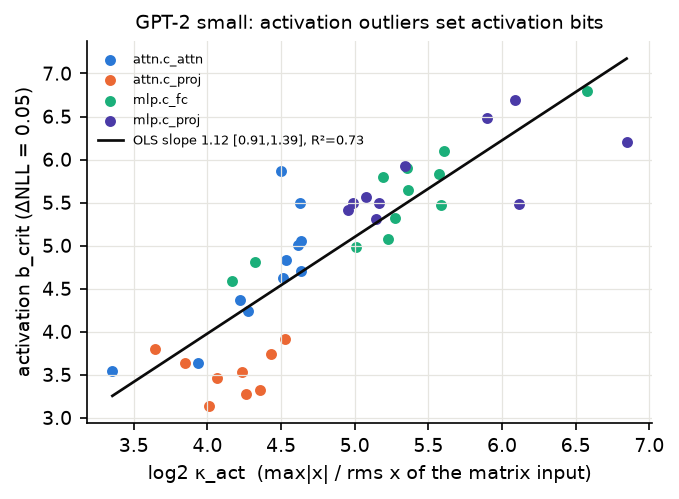
\includegraphics[width=0.6\linewidth]{fig12_activation_kappa.png}
\caption{GPT-2 small: per-matrix activation bit-width against the activation outlier ratio.}\label{fig:act}\end{figure}
\emph{Mixed precision:} allocations at equal parameter-weighted budgets on held-out tokens
(Table~\ref{tab:mixed}). \emph{Tokens:} per-token fp32 logit margin and survival under joint quantization.
\emph{SAE:} \texttt{jbloom/GPT2-Small-SAEs-Reformatted}, \texttt{blocks.6.hook\_resid\_pre}, applied to the
mean-centred HF residual stream with the decoder bias subtracted (84\,\% variance explained, $L_0\approx58$; the
alternatives give $<0$); 196{,}596 tokens in 128-token BOS-prefixed contexts; feature retention
$\rho_f = 1-\sum_t(a_f^q-a_f^{\mathrm{fp32}})^2/\sum_t(a_f^{\mathrm{fp32}})^2$; live if firing on $\ge20$ tokens.
\begin{table}[h]\centering\small
\caption{Mixed precision on GPT-2 small: $\Delta$NLL (nats, held-out) at equal average bits.}
\label{tab:mixed}
\begin{tabular}{lccccc}\toprule
avg.\ bits & uniform & $\kappa$-rule & noise-probe law & oracle & random ($\times3$)\\\midrule
3.5 & -- & 3.56 & \textbf{1.86} & 2.08 & 3.6--4.1\\
4.0 & \textbf{0.449} & 0.659 & 0.600 & 0.459 & 0.68--0.88\\
4.5 & -- & 0.274 & \textbf{0.190} & 0.183 & 0.26--0.33\\
5.0 & \textbf{0.084} & 0.094 & 0.103 & 0.067 & 0.10--0.11\\\bottomrule
\end{tabular}
\end{table}

\section{Preregistration scoring and dated deviations}
\label{app:score}
\label{app:deviations}
\begin{center}\small
\resizebox{\linewidth}{!}{\begin{tabular}{p{4.6cm}p{3.6cm}p{5.6cm}}\toprule
prediction & rule & outcome\\\midrule
P1: slope $\nicefrac12$ in $\log_2F$ & $[0.4,0.6]$ / $[0.15,0.35]$ / $<0.15$ & \textbf{dead}: $-0.11$ (QAT), $+0.03$ (PTQ), all definitions $<0.15$\\
P2: $\kappa$ enters as $\log_2\kappa$, slope 1 & $[0.7,1.3]$ / $\approx0$ / partial & \textbf{partial, strong}: $0.65$ ($R^2$ 0.92), $0.72$, $0.63$\\
P3: ordering preserved (power-law $I$) & prefix drop $<0.10$ & \textbf{confirmed}: $\le0.03$\\
E3: noise-like slope $-\nicefrac12$; structured $\approx0$ & & noise-like $\approx0$; dropout $+0.24$; rank catastrophic\\
E4: top features unchanged & drop $<0.05$ & tilt, not translation (uniform $I$)\\
LM: $\log_2\sigma_{\mathrm{crit}}$ vs $\log_2\hat F\in[-0.65,-0.35]$ & & \textbf{not}: $+0.14$ [$-0.13$, $0.35$]\\
D2 (pre-E1): $\sigma_{\mathrm{crit}}$ flat, $b=\mathrm{const}+\log_2\kappa$ & & \textbf{confirmed}\\\bottomrule
\end{tabular}}
\end{center}
Deviations (dated in the repository): D1, after the fp32-only gate, the hard count made continuous; D2, after the sizing
pilot and before the main sweep, the corrected derivation and its decision rule; D3, after a pilot damage run, clipping
bias and dead-feature accounting fixed by $R_{\mathrm{live}}$ with paired evaluation; D4, after an external review of the
draft, the activation arm added as a post-hoc application of P2's functional form to a new quantity (not preregistered
coverage), and the per-token and SAE analyses recorded as exploratory.

\section{Additional figures}
\begin{figure}[h]\centering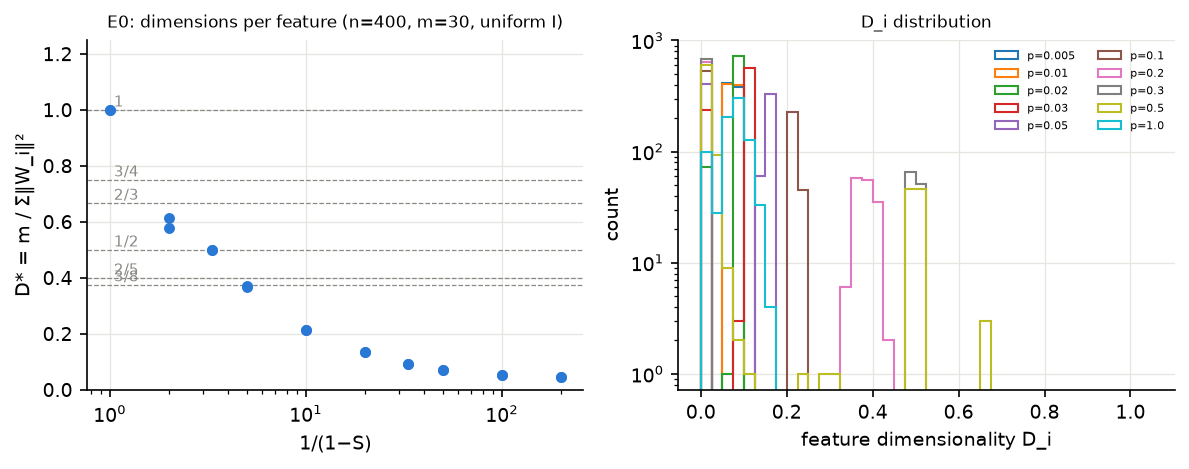
\includegraphics[width=0.85\linewidth]{fig0_e0_replication.png}
\caption{E0: fp32 replication of the feature-dimensionality ladder.}\label{fig:e0}\end{figure}
\begin{figure}[h]\centering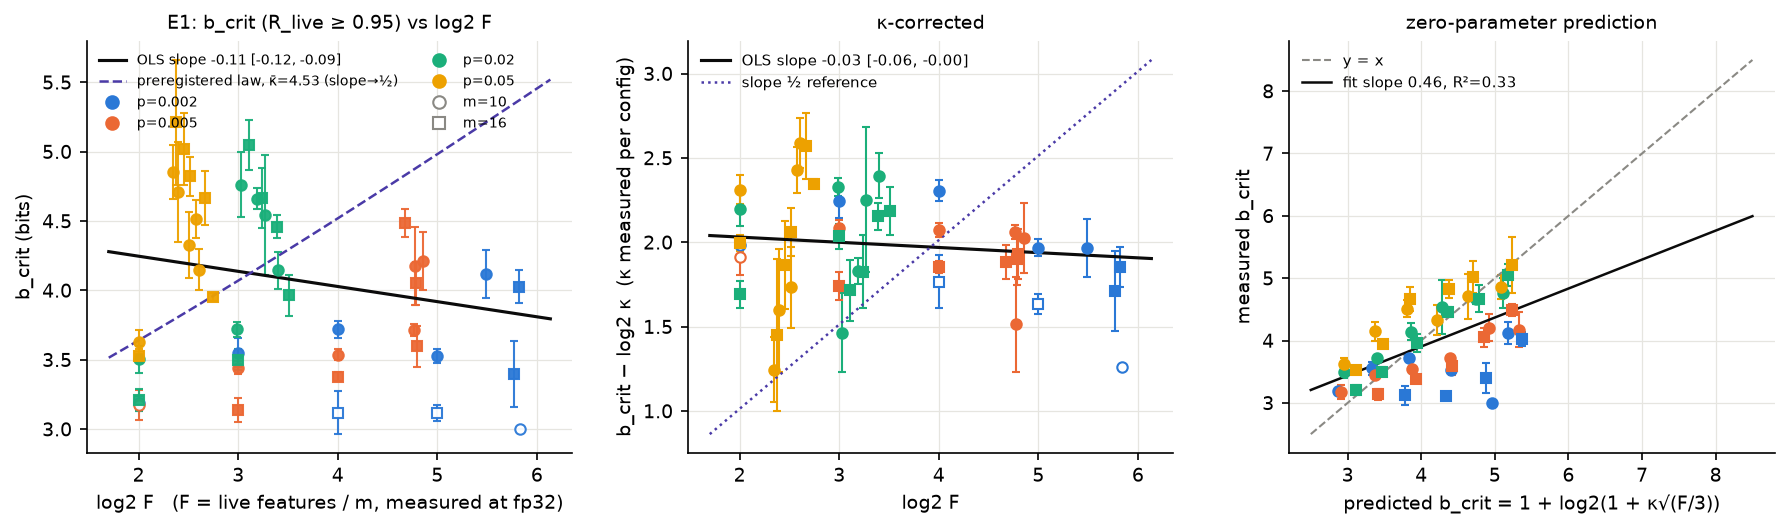
\includegraphics[width=\linewidth]{fig1_bcrit_vs_F_R_live_95.png}
\caption{E1 money plot with $\kappa$-corrected and zero-parameter panels.}\end{figure}
\begin{figure}[h]\centering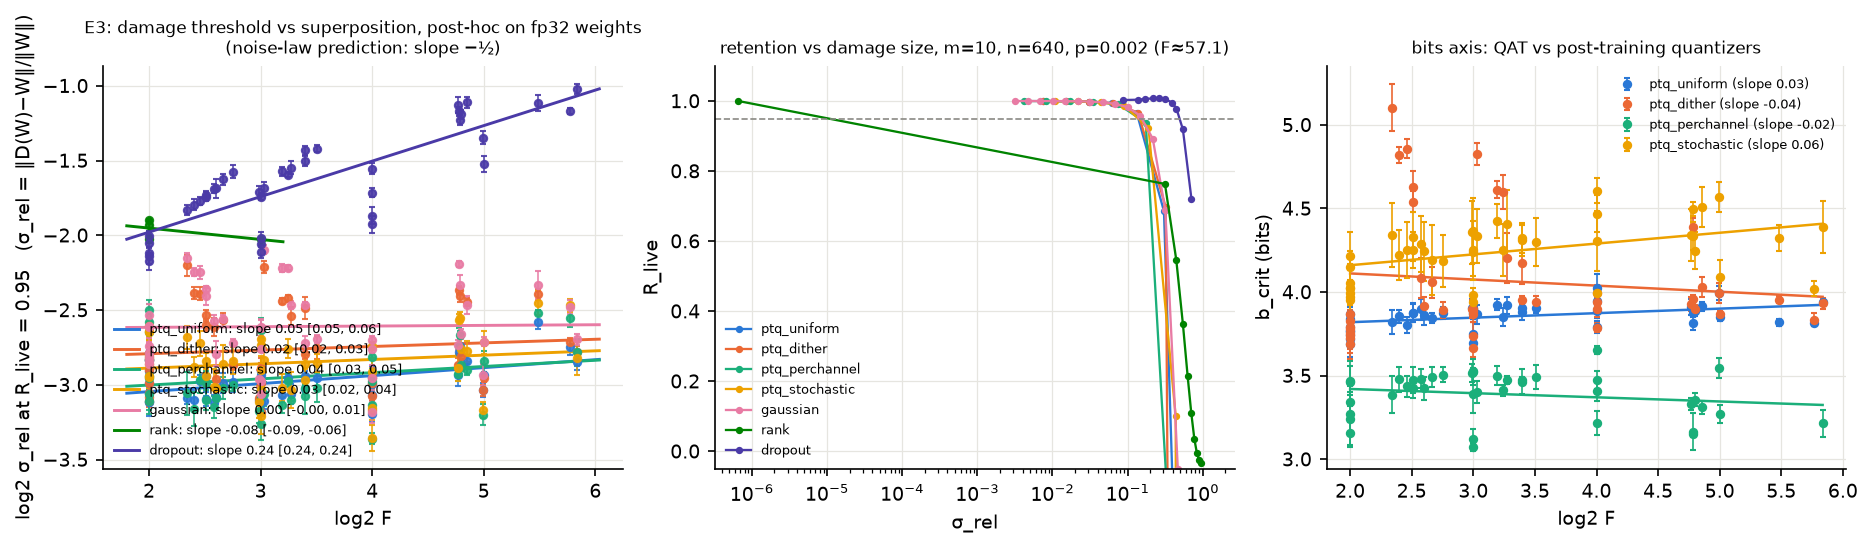
\includegraphics[width=\linewidth]{fig3_anydamage_null.png}
\caption{E3: seven damage families on a common $\sigma_{\mathrm{rel}}$ axis.}\end{figure}
\begin{figure}[h]\centering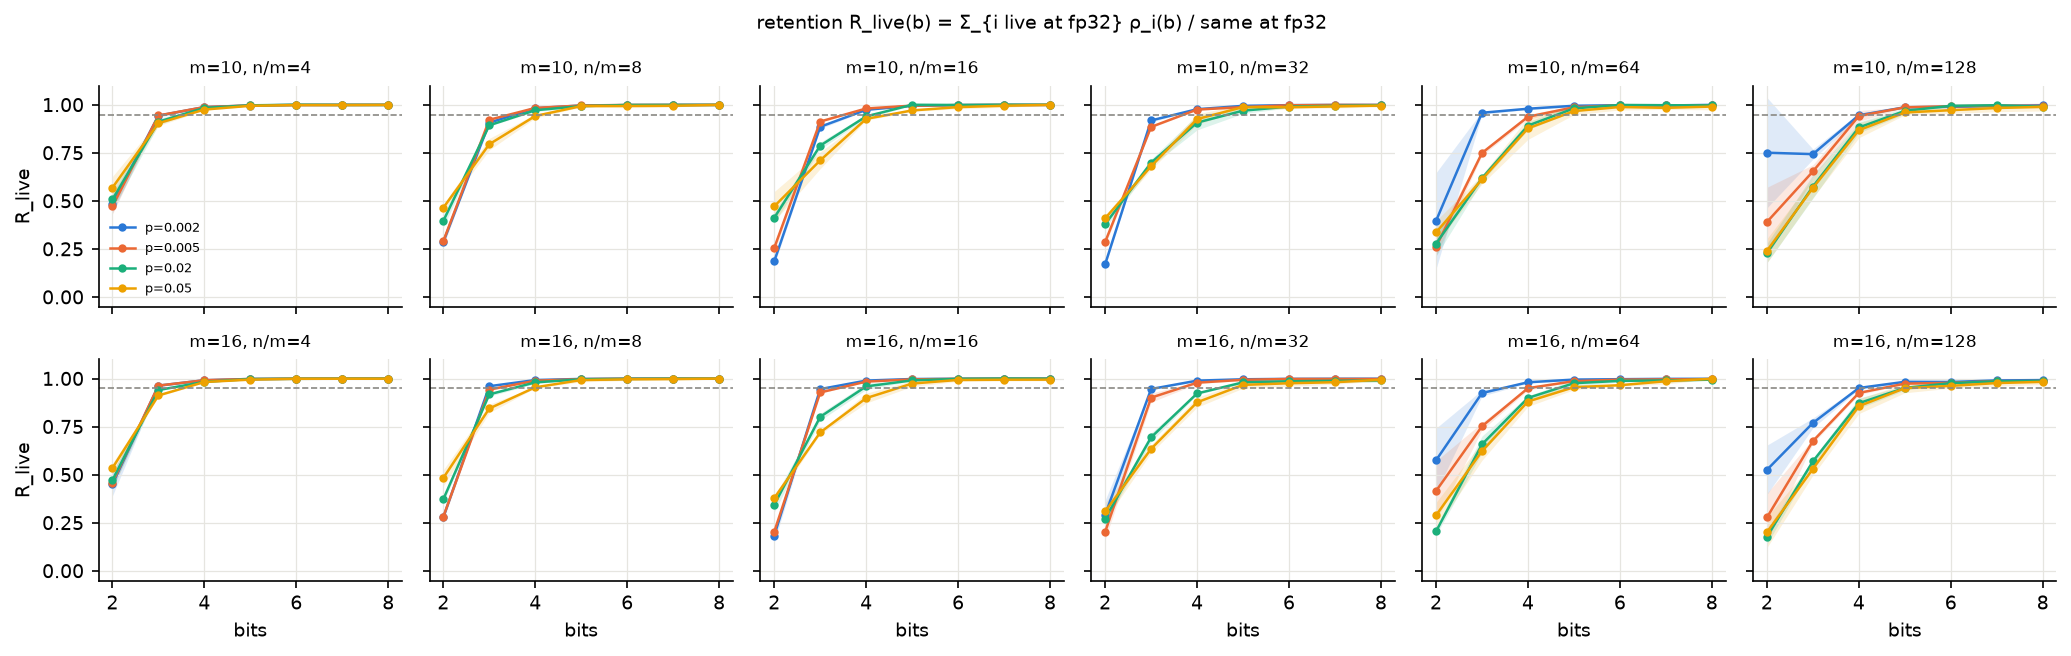
\includegraphics[width=\linewidth]{fig2_Nret_vs_bits.png}
\caption{E1 retention curves for every cell.}\end{figure}
\begin{figure}[h]\centering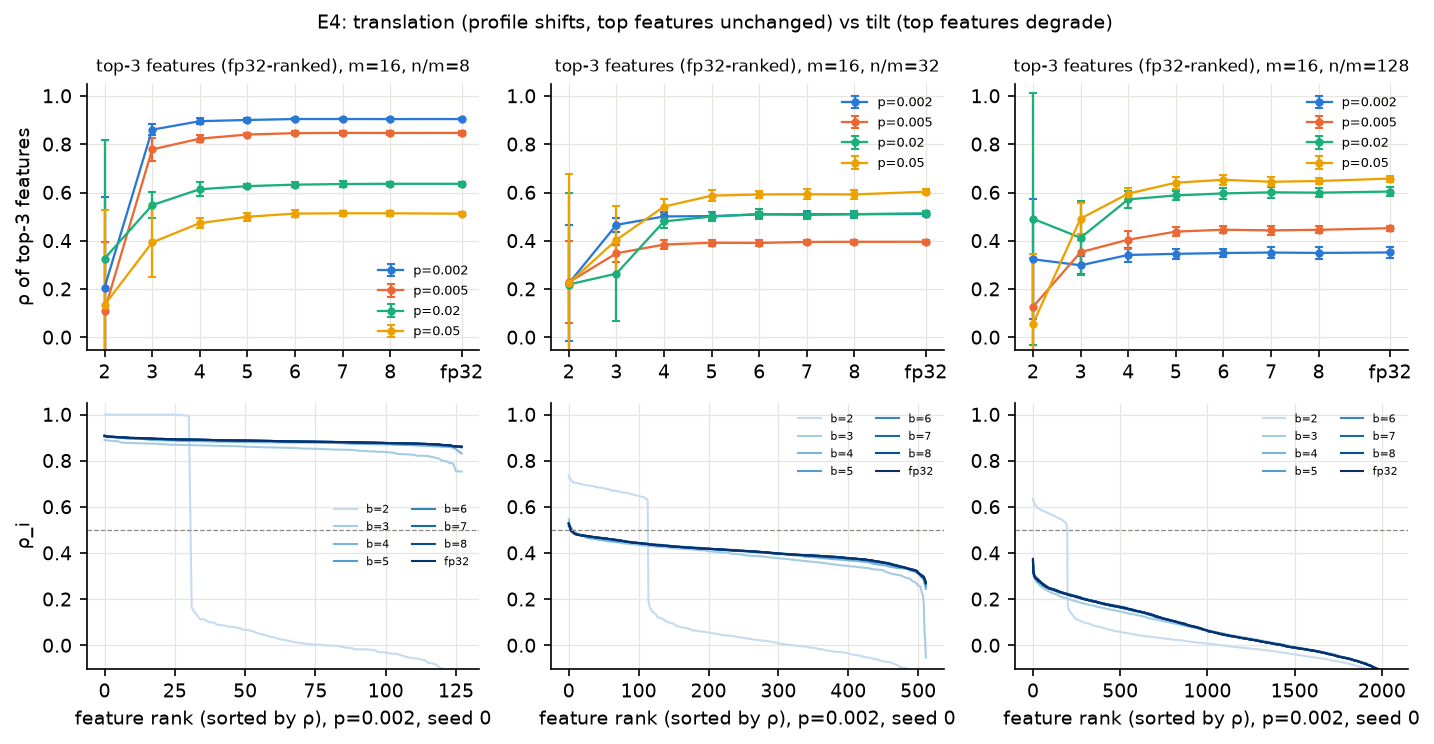
\includegraphics[width=\linewidth]{fig4_translation_vs_tilt.png}
\caption{E4: top-3 feature $\rho$ against bit-width and sorted $\rho$ profiles.}\end{figure}
\begin{figure}[h]\centering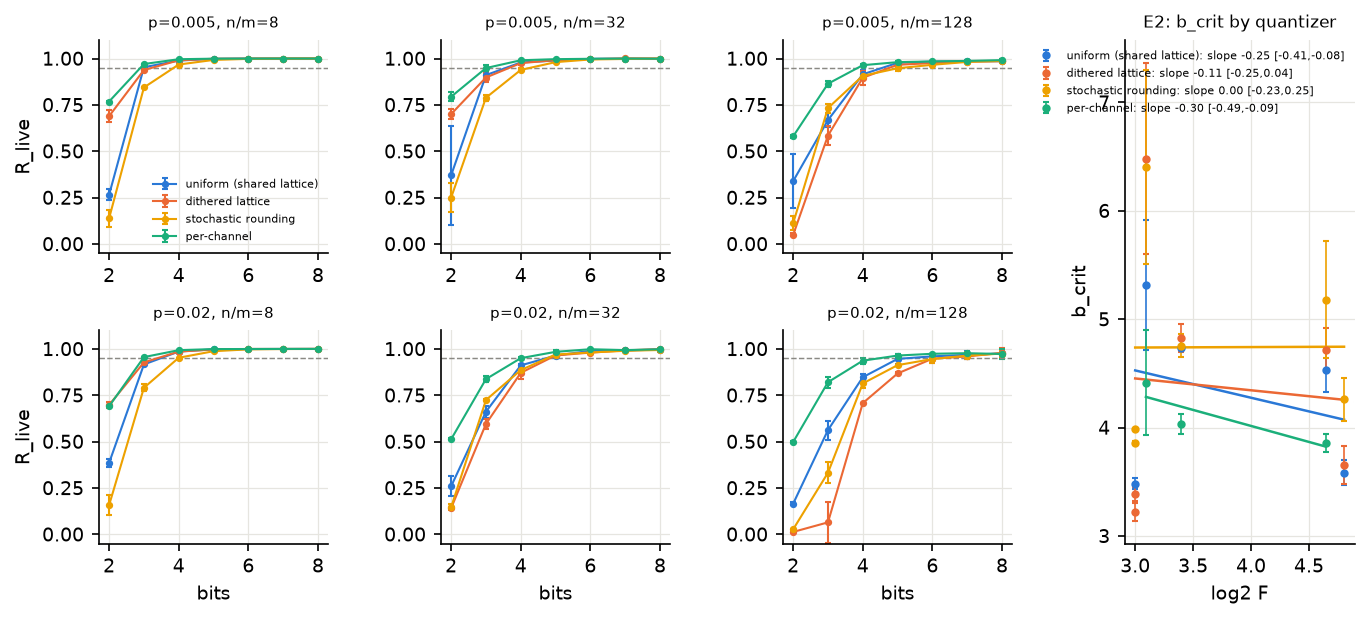
\includegraphics[width=\linewidth]{fig5_lattice.png}
\caption{E2: quantizers under QAT.}\end{figure}
\begin{figure}[h]\centering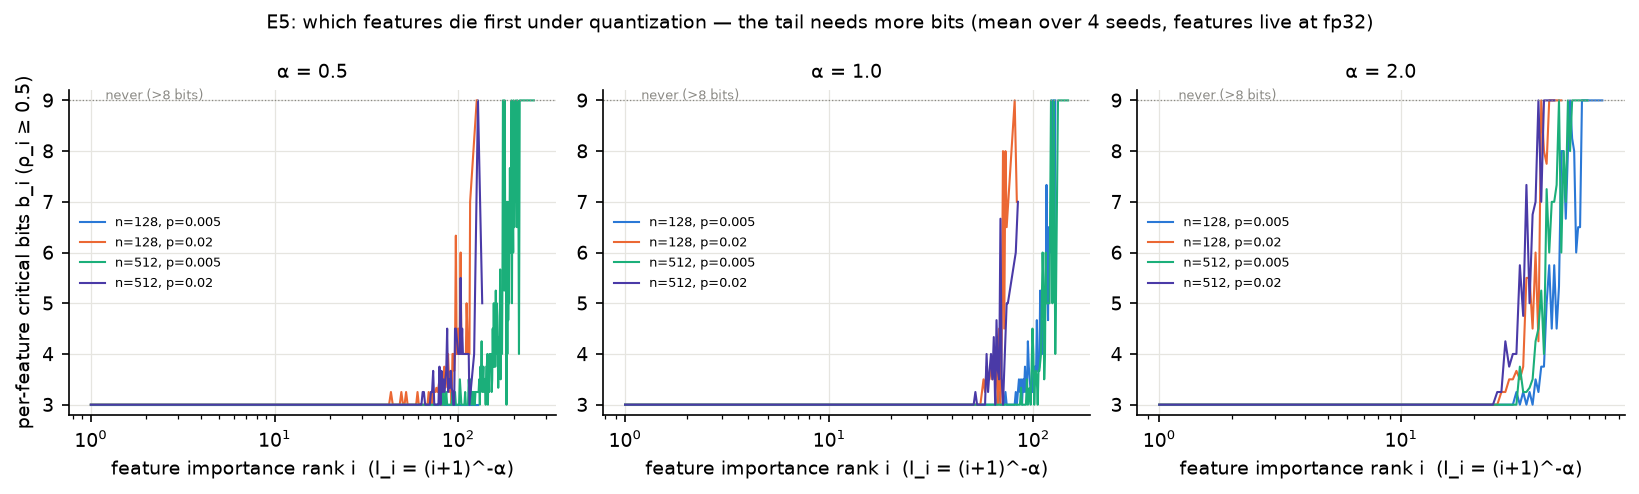
\includegraphics[width=\linewidth]{fig6b_per_feature_bits.png}
\caption{E5: per-feature critical bits against importance rank.}\end{figure}
\begin{figure}[h]\centering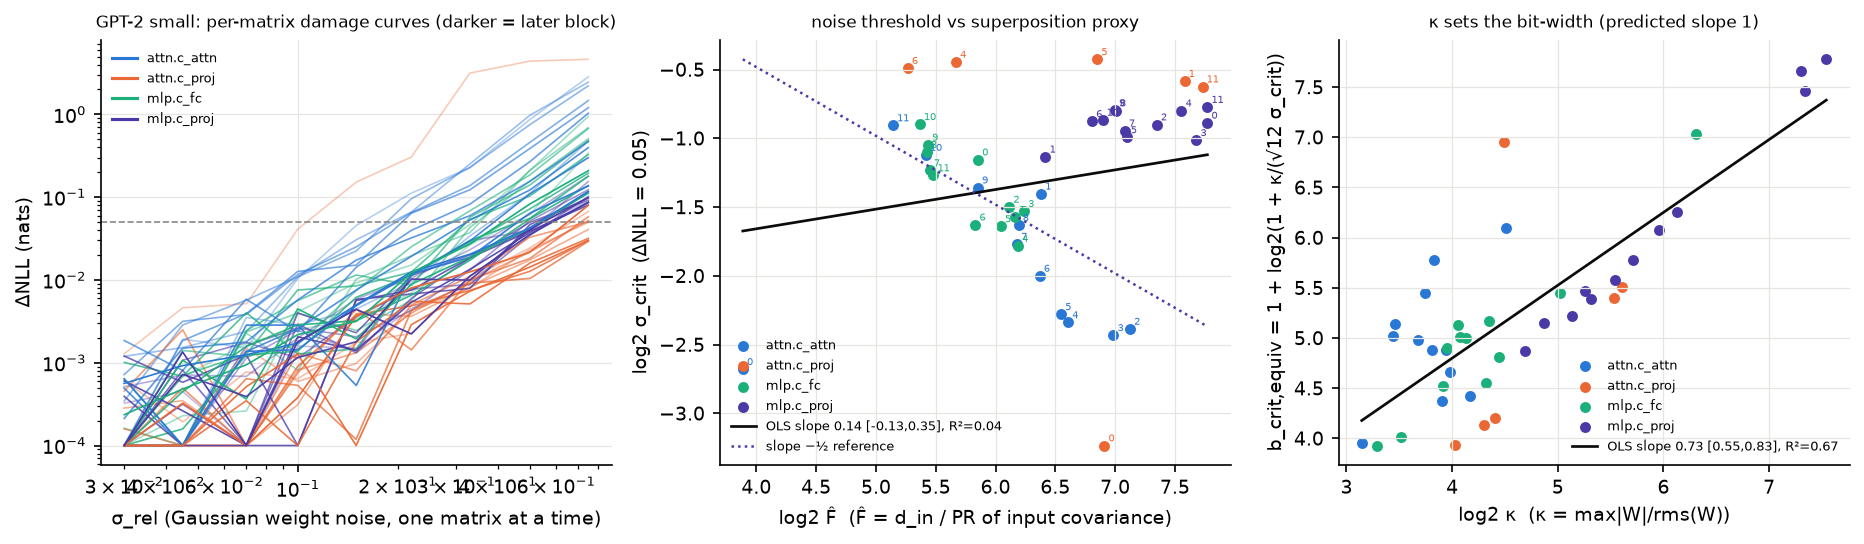
\includegraphics[width=\linewidth]{fig7_lm_layers.png}
\caption{GPT-2 per-matrix damage curves, noise threshold vs $\hat F$, and bit-equivalent vs $\kappa$.}\end{figure}
\begin{figure}[h]\centering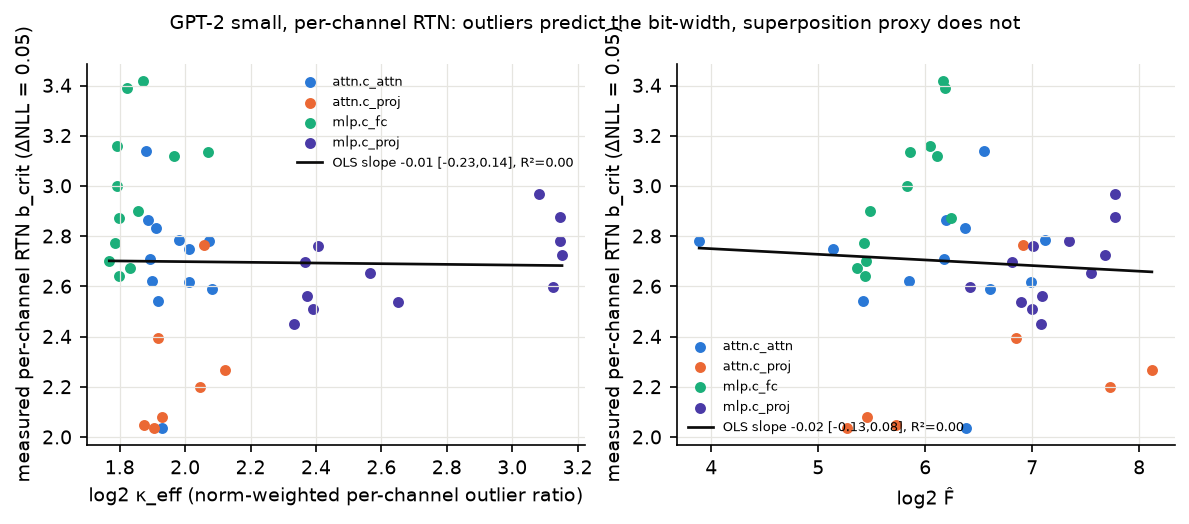
\includegraphics[width=0.8\linewidth]{fig7b_lm_perchannel.png}
\caption{GPT-2 per-channel RTN: all matrices at $2.7\pm0.3$ bits.}\end{figure}
\begin{figure}[h]\centering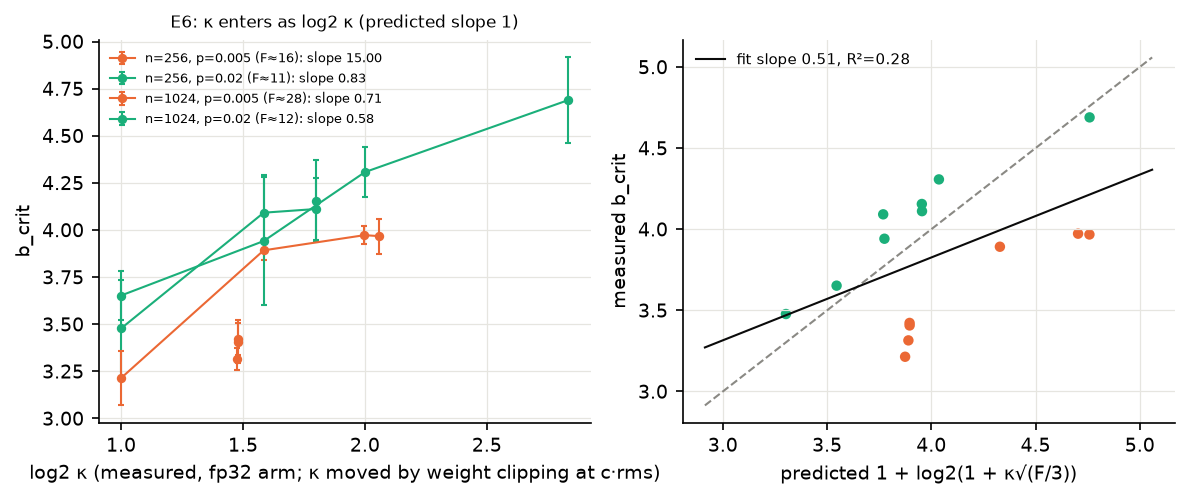
\includegraphics[width=0.85\linewidth]{fig8_kappa.png}
\caption{E6: $\kappa$ moved by clipping.}\end{figure}
\begin{figure}[h]\centering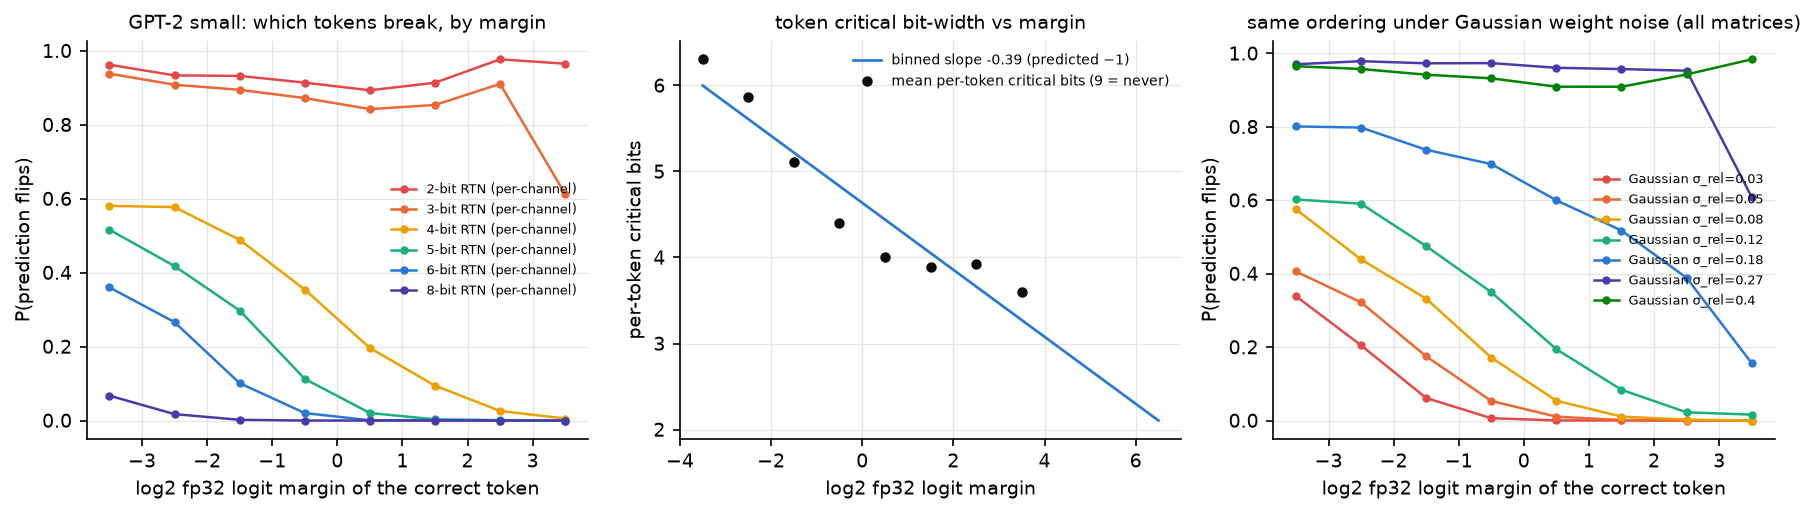
\includegraphics[width=\linewidth]{fig10_token_margins.png}
\caption{GPT-2 tokens: flip probability by margin, critical bits vs margin, Gaussian control.}\end{figure}
\begin{figure}[h]\centering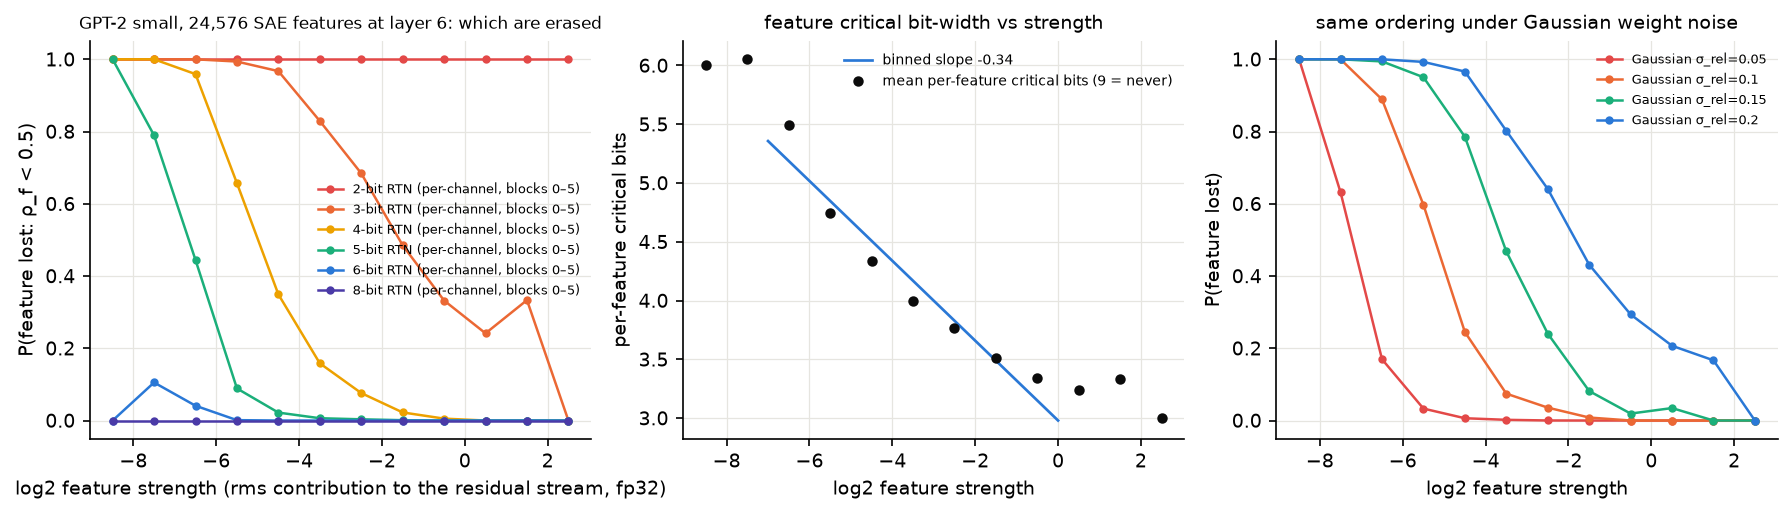
\includegraphics[width=\linewidth]{fig11_sae_features.png}
\caption{GPT-2 SAE features: loss by strength, critical bits vs strength, Gaussian control.}\end{figure}

\section{Declaration of LLM and agent usage}
\label{app:llm}
The experiments, analysis code and first drafts of this paper were implemented and executed by an AI coding agent
(Claude Code) under the direction of the authors, following a written, preregistered experimental plan; the authors
specified the hypotheses, decision rules and controls, reviewed every analysis choice recorded in the deviations log, and
verified the reported numbers against the raw results. This is a non-standard component of the methodology and is
declared per the NeurIPS 2026 policy.

\section*{NeurIPS Paper Checklist}
\begin{enumerate}
\item {\bf Claims} \\ Question: Do the main claims made in the abstract and introduction accurately reflect the paper's contributions and scope? \\ Answer: \answerYes{} \\ Justification: Every number in the abstract and contribution list is reported with its CI or $R^2$ in Sec.~3 and App.~C, including the preregistered predictions that failed.
\item {\bf Limitations} \\ Question: Does the paper discuss the limitations of the work performed by the authors? \\ Answer: \answerYes{} \\ Justification: Sec.~5 (single tied layer, criterion-dependent $\sigma^*$, crude superposition proxy, one LM/corpus/SAE layer, sub-unit $\kappa$ slope, metric change from the preregistration).
\item {\bf Theory assumptions and proofs} \\ Question: For each theoretical result, does the paper provide the full set of assumptions and a complete (and correct) proof? \\ Answer: \answerNA{} \\ Justification: The derivations are heuristic scaling arguments with their assumptions stated (unit live columns, Welch-bound interference, uniform residual); no theorem is claimed and the paper tests the predictions empirically.
\item {\bf Experimental result reproducibility} \\ Question: Does the paper fully disclose all the information needed to reproduce the main experimental results? \\ Answer: \answerYes{} \\ Justification: App.~A--B give model, training, quantizer, metric, data, SAE and evaluation details; the preregistration and all per-model results accompany the code.
\item {\bf Open access to data and code} \\ Question: Does the paper provide open access to the data and code? \\ Answer: \answerYes{} \\ Justification: Anonymized code, preregistration, deviation log and per-model result tables are provided as supplementary material and will be released publicly; GPT-2, WikiText-2 and the SAE are public.
\item {\bf Experimental setting/details} \\ Question: Does the paper specify all the training and test details? \\ Answer: \answerYes{} \\ Justification: App.~A (optimizer, schedule, batch, steps, initialisation, evaluation sample counts) and App.~B (token budgets, offsets, thresholds, SAE conventions).
\item {\bf Experiment statistical significance} \\ Question: Does the paper report error bars or other appropriate information about statistical significance? \\ Answer: \answerYes{} \\ Justification: Seed SDs on every toy point, seed-bootstrap 95\,\% CIs on every slope, matrix-bootstrap CIs and $R^2$ for GPT-2 regressions, paired SEMs for quantizer contrasts.
\item {\bf Experiments compute resources} \\ Question: Does the paper provide sufficient information on the computer resources? \\ Answer: \answerYes{} \\ Justification: App.~A: about four GPU-hours on one 24\,GB M-series laptop for all experiments.
\item {\bf Code of ethics} \\ Question: Does the research conform with the NeurIPS Code of Ethics? \\ Answer: \answerYes{} \\ Justification: Public models and data only; no human subjects.
\item {\bf Broader impacts} \\ Question: Does the paper discuss both potential positive and negative societal impacts? \\ Answer: \answerNA{} \\ Justification: Foundational work on when quantization erases representations; it can make compression more predictable and has no direct path to misuse.
\item {\bf Safeguards} \\ Question: Does the paper describe safeguards for responsible release of high-risk assets? \\ Answer: \answerNA{} \\ Justification: No models or datasets are released.
\item {\bf Licenses for existing assets} \\ Question: Are the creators of assets properly credited and licenses respected? \\ Answer: \answerYes{} \\ Justification: GPT-2 (MIT, via Hugging Face), WikiText-2 (CC BY-SA 3.0), the GPT-2 SAEs of \cite{bloom2024sae} (public release), all cited.
\item {\bf New assets} \\ Question: Are new assets well documented? \\ Answer: \answerYes{} \\ Justification: The code base ships with a README, tests and a per-experiment registry.
\item {\bf Crowdsourcing and research with human subjects} \\ Answer: \answerNA{} \\ Justification: None.
\item {\bf Institutional review board (IRB) approvals} \\ Answer: \answerNA{} \\ Justification: No human subjects.
\item {\bf Declaration of LLM usage} \\ Question: Does the paper describe the usage of LLMs if it is an important, original, or non-standard component of the core methods? \\ Answer: \answerYes{} \\ Justification: App.~E declares that an AI coding agent implemented and executed the experiments and analysis under the authors' direction and preregistered plan.
\end{enumerate}

\end{document}
